\RequirePackage[l2tabu, orthodox]{nag}
\documentclass{standalone}

\usepackage{tikz}
\usetikzlibrary{shapes.geometric}
%\usetikzlibrary{decorations.text}
%\usetikzlibrary{knots}
\usetikzlibrary{calc}
\usetikzlibrary{intersections}

\begin{document}

\newcommand{\nfoil}[4][]{
  \node [minimum size=#3, regular polygon, regular polygon sides=#2] at (0,0) (E) {};
  \node [minimum size=#4, regular polygon, regular polygon sides=#2] at (0,0) (I) {};
  \foreach \i in {1,...,#2} {
    \pgfmathtruncatemacro{\pp} {mod(#2+\i-3,#2)+1}
    \pgfmathtruncatemacro{\p}  {mod(#2+\i-2,#2)+1}
    \pgfmathtruncatemacro{\s}  {mod(   \i  ,#2)+1}
    \pgfmathtruncatemacro{\ss} {mod(   \i+1,#2)+1}
    \pgfmathtruncatemacro{\sss}{mod(   \i+2,#2)+1}
    \path[name path=s-I-sss] (I.corner \s) -- (I.corner \sss);
    \path[name path=i-I-ss]  (I.corner \i) -- (I.corner \ss);
    \path[name path=i-I-pp]  (I.corner \i) -- (I.corner \pp);
    \path[name path=i-E-pp]  (E.corner \i) -- (E.corner \pp);
    \path[name path=i-E-ss]  (E.corner \i) -- (E.corner \ss);
    \path[name path=p-E-s]   (E.corner \p) -- (E.corner \s);
    \node[coordinate, name intersections = {of=i-E-ss and s-I-sss}] (Es) at (intersection-1) {};
    \node[coordinate, name intersections = {of=i-I-ss and s-I-sss}] (Is) at (intersection-1) {};
    \node[coordinate, name intersections = {of=i-E-pp and p-E-s}]   (Ep) at (intersection-1) {};
    \node[coordinate, name intersections = {of=i-I-pp and p-E-s}]   (Ip) at (intersection-1) {};
    \draw[#1] (Ep) -- (E.corner \i) -- (Es);
    \draw[#1] (Ip) -- (I.corner \i) -- (Is);
  }
}

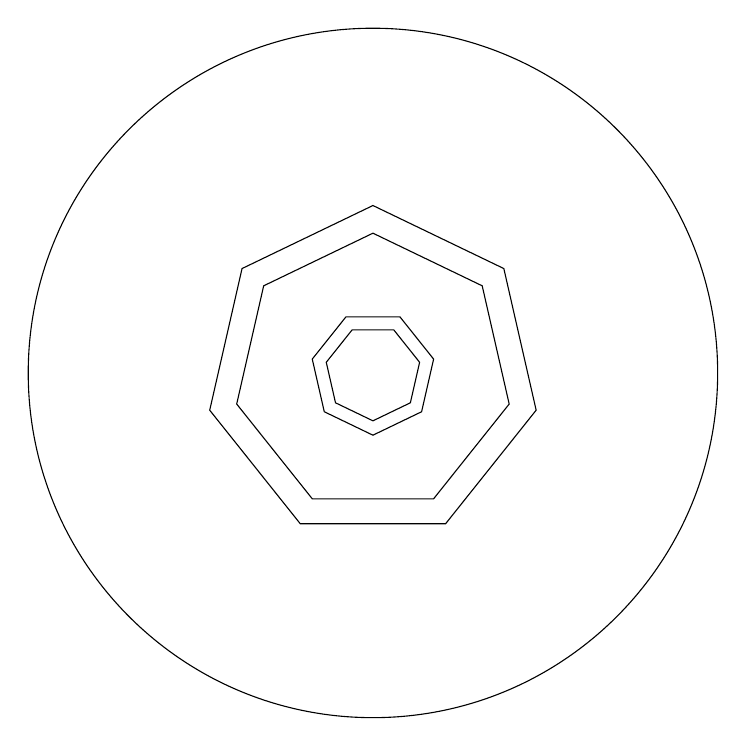
\begin{tikzpicture}

\nfoil[]{7}{100pt}{80pt}
\nfoil[]{5}{30pt}{20pt}

\def\ro{0.69202147163}%internal

\node [rotate=180, draw, minimum size=65pt*\ro, regular polygon, regular polygon sides=7] at (0,0) () {};
\node [rotate=180, draw, minimum size=50pt*\ro, regular polygon, regular polygon sides=7] at (0,0) () {};
\node [draw, minimum size=101, regular polygon, regular polygon sides=7] at (0,0) () {};
\node [draw, minimum size=121pt, regular polygon, regular polygon sides=7] at (0,0) () {};
\draw (0,0) circle (180pt*\ro);
\end{tikzpicture}











\end{document}
